\documentclass[t]{beamer}

\usetheme{Boadilla}

\usepackage[T1]{fontenc}
\usepackage{graphicx}
\usepackage{pict2e}
\usepackage{xcolor}
\usepackage{amsmath}
\usepackage[rflt]{floatflt}
\usepackage{graphicx,subfigure,epic,eepic}
\usepackage[most]{tcolorbox}
\usepackage{float}
\usepackage{caption}
\usepackage{fullpage}
\usepackage{hyperref}





\title{Canalising strength of a node in emt networks}
\author{Vaibhav Anand}

\begin{document}


\begin{frame}
\titlepage
\end{frame}


\begin{frame}
\frametitle{Canalizing strength of a node}

We define a metric called canalizing strength of a node as  \[  |\mu_{excitatory} - \mu_{inhibitory}|                    \]

It is the absolute difference in the number of excitatory and inhibitory outgoing connections of a node. Nodes which have more outgoing edges of a similar nature acts uniformly on other nodes compared to nodes having edges of different natures, such nodes can have more number of outcomes for an input.  
\end{frame}


\begin{frame}
	\frametitle{EMT networks have high mean canalizing value}

	Upon random swapping of edges (10 at a time) so that the in and out degree of a node is constant, it was found that the wild type network has higher mean than most random networks. 



\end{frame} 


\begin{frame}
	\begin{figure}[H]
	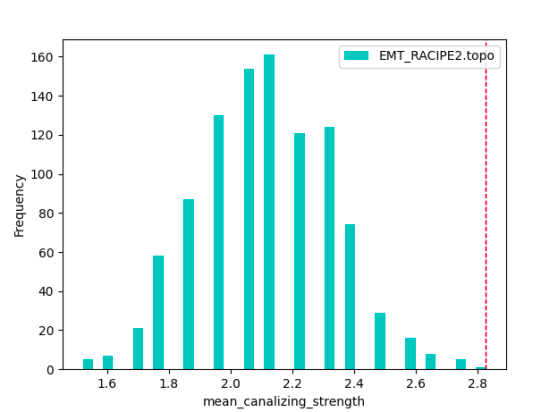
\includegraphics[scale=0.4]{img/emt_racipe_1.png}
	\caption{Distribution of mean}
	\end{figure}
\end{frame}

\begin{frame}
\begin{figure}[H]
	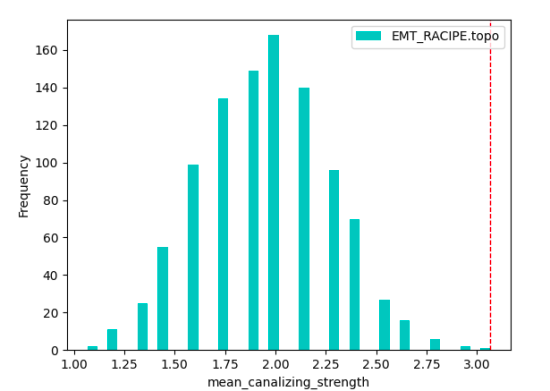
\includegraphics[scale=0.4]{img/emt_racipe_2.png}
	
\end{figure}


\end{frame}

\begin{frame}
	\begin{figure}[H]
		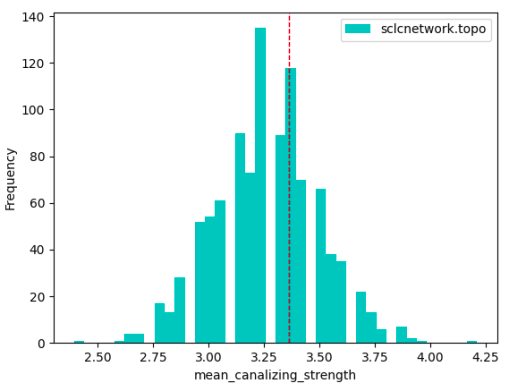
\includegraphics[scale=0.4]{img/melanoma_outcan.png}
		\caption{sclcnetwork }
	\end{figure}

\end{frame}


\begin{frame}
	\frametitle{Knockout Of Nodes}
	Since in the networks concerned there aren't many nodes, node knockout analysis did not allow for elimination of several confounding factors like high indegree etc. No consistent results were obtained on node knockout

\end{frame}

\begin{frame}
	\frametitle{Steady states without any node knockout}
	\begin{figure}[H]
		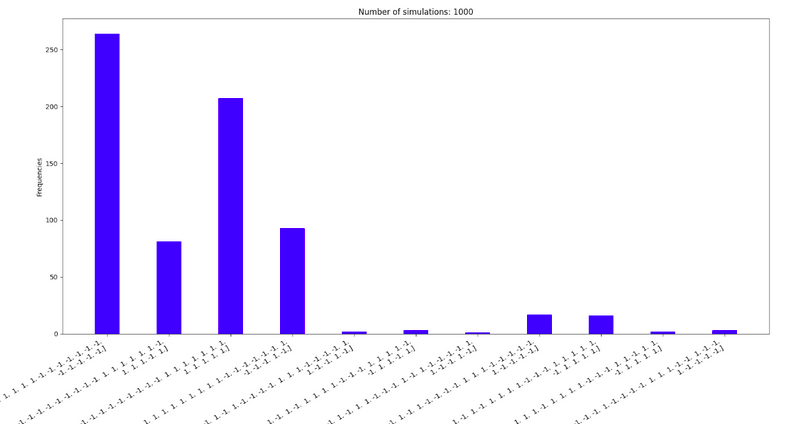
\includegraphics[scale=0.3]{img/normalemtracipe.png}
			\end{figure}
\end{frame}

\begin{frame}
	\frametitle{Steady states after knockout of a node with canalising value 3}
	\begin{figure}[H]
		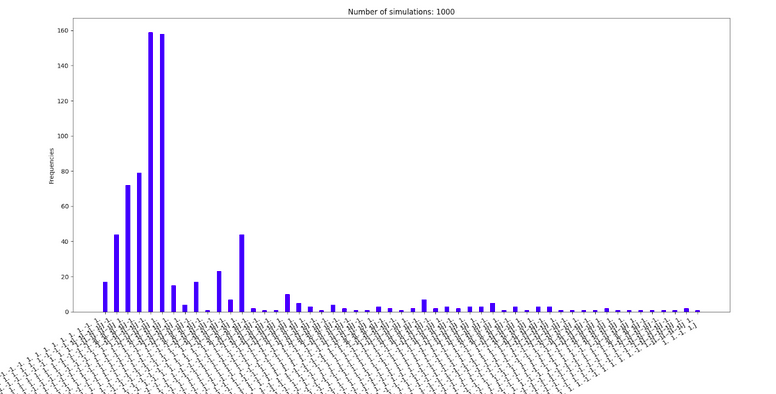
\includegraphics[scale=0.25]{img/nodeknockout.png}
		\caption{Destabilizing}
			\end{figure}
\end{frame}


\begin{frame}
	\frametitle{ Steady states after knockout of a different node with canalising value 3}
	\begin{figure}[H]
		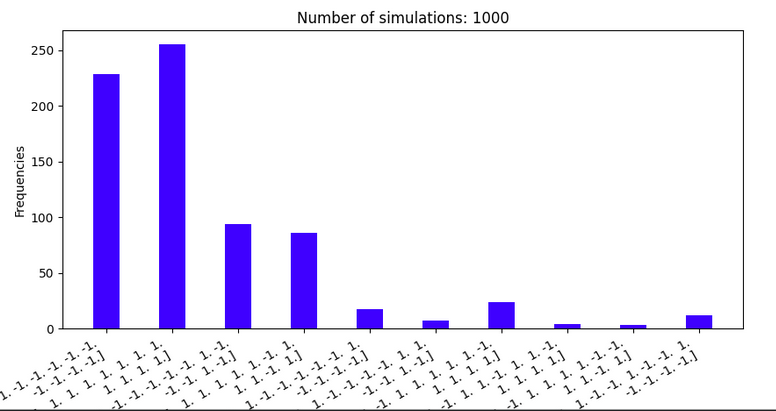
\includegraphics[scale=0.25]{img/node3emtracipe2outcan3incani.png}
		\caption{Stabilizing}
			\end{figure}
\end{frame}



\begin{frame}
	\frametitle{Boolean Formalism}
	The rules of boolean formalims are as follows. 
	
	\begin{item}
\item $ S_j = 1 $ if    $  \sum_{ i } ^ { } adj[i][j] * S_i> 0 $ 

	\item $ S_j = -1 $ if    $  \sum_{ i } ^ { } adj[i][j] * S_i< 0 $

	\item $ S_j = S_j  $ if   $  \sum_{ i } ^ { } adj[i][j] * S_i= 0$ 
	\item In the case where the above sum is 0 we let the node have whatever state it had before and be somewhat `unregulated'	
	\end{item}
\end{frame}


\begin{frame}
	\frametitle{Steady states using boolean formalism}
	\begin{figure}[H]
	
		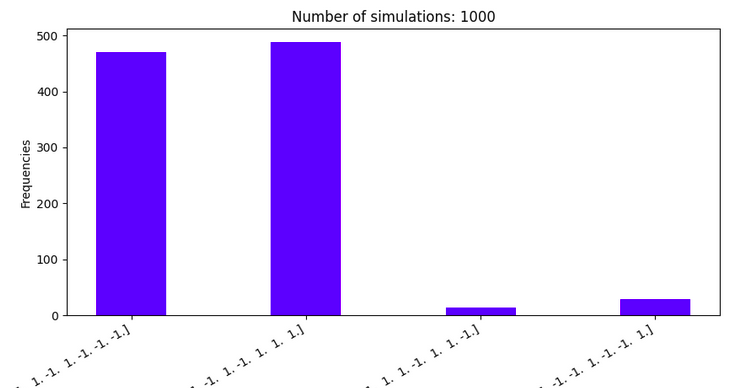
\includegraphics[scale=0.3]{img/emtracipebool.png}
		\caption{EMT Network 15 nodes}
	\end{figure}
\end{frame}

\begin{frame}
\begin{figure}[H]
	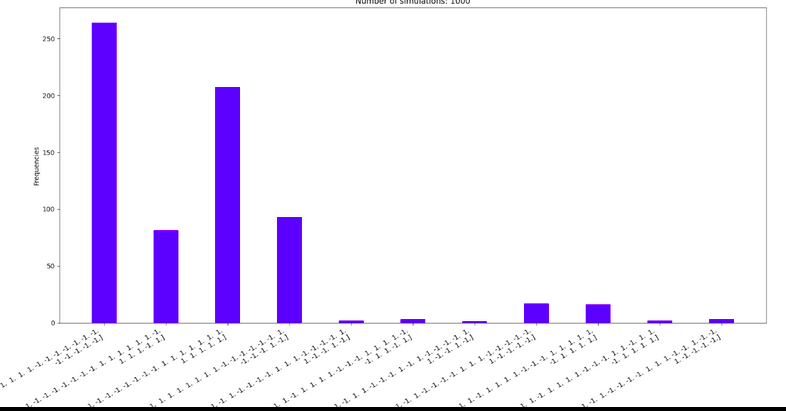
\includegraphics[scale=0.3]{img/emtracipe2bool.png}
	\caption{EMT Network 23 nodes}
\end{figure}
\end{frame}

\begin{frame}
	\frametitle{Dynamic InCanalising Strength}

	It quantifies how much activating or inhibhiting regulation and node is under at a certain time step. It is defined as follows for the J'th node
\[   \sum_{ i } ^ { } adj[i][j] * S_i                    \]
Here, $ S_i $ denotes the state of I'th node and adj refers to the adjacency matrix of the network 
\end{frame}

\begin{frame}
	\frametitle{Distribution of absolute InCan value for an extremal state(epithelial or mesenchymal}

	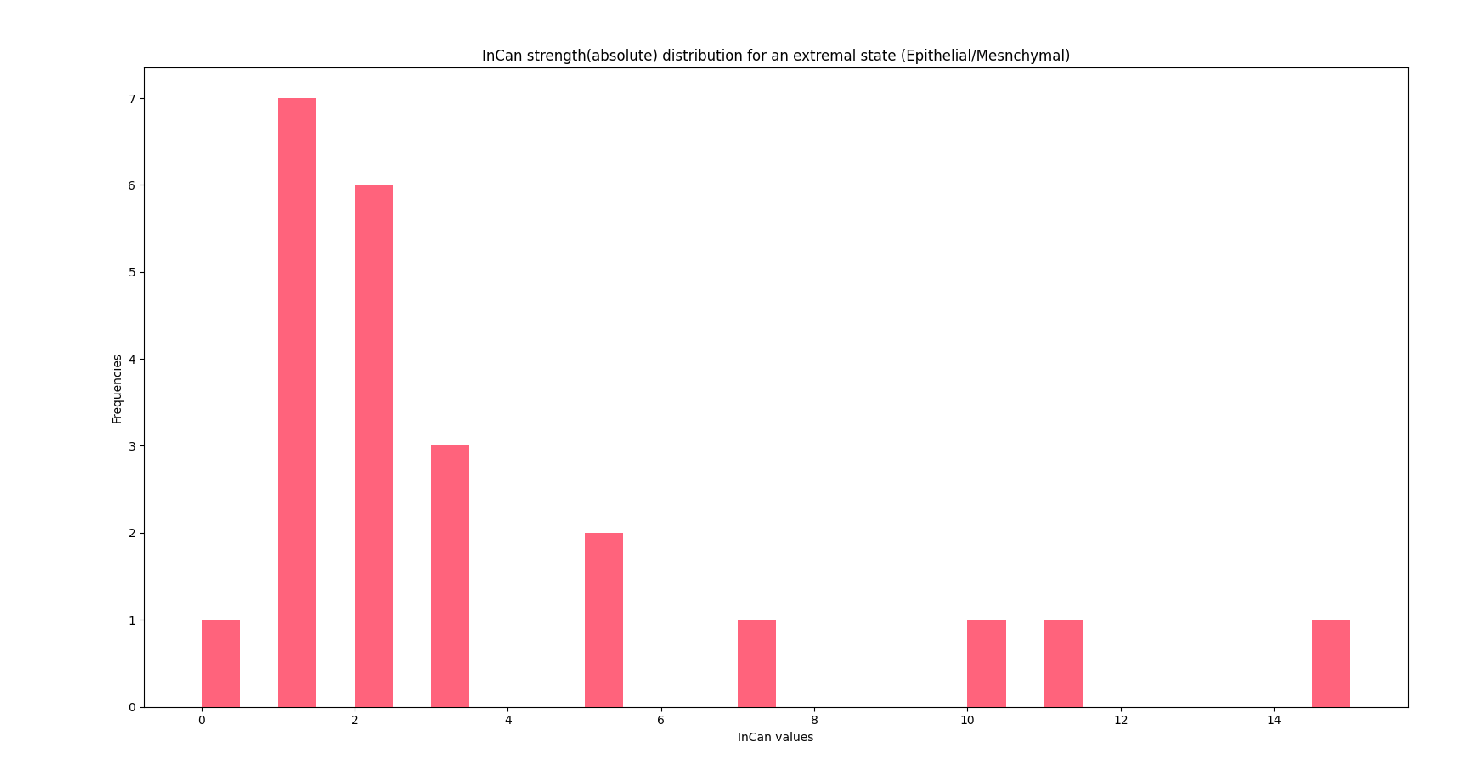
\includegraphics[scale=0.17]{img/incan_epi_emtracipe2.png}
	\end{frame}

\begin{frame}
	\frametitle{Hybrid States have more nodes with lesser InCan value indicating "lesser regulation"}
\begin{figure}[H]
	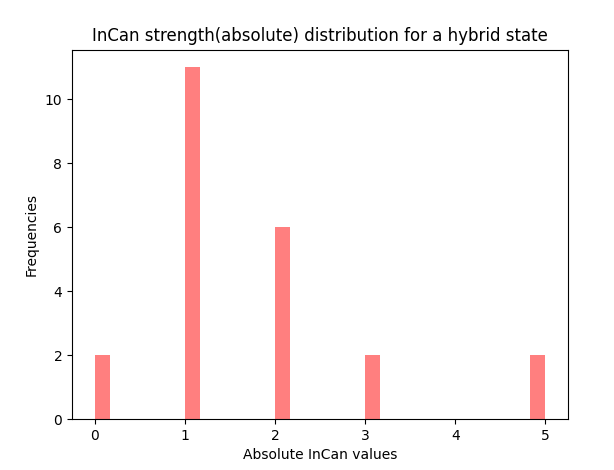
\includegraphics[scale=0.25]{img/hybrid_incan_emtracipe2.png}
	\end{figure}
\end{frame}

\begin{frame}
	\frametitle {Three State Formalism}
	The three state formalism with the following rules renders the node with canalising strength 0 incapable of any forward regulation and affecting the state of other nodes at each time step.
	\begin{item}
	\item $ S_j = 1 $ if    $  \sum_{ i } ^ { } adj[i][j] * S_i> 0 $

	\item $ S_j = -1 $ if    $  \sum_{ i } ^ { } adj[i][j] * S_i< 0 $

	\item $ S_j = 0 $ if    $  \sum_{ i } ^ { } adj[i][j] * S_i= 0 $


	\end{item}
	\end{frame}

\begin{frame}
	\frametitle{Results using three state formalism}
	Upon using the three state formalism which dynamically sets the expression level of the the nodes having incan strength 0 and renders them incapable of any forward regulation. We find that upon using this formalism all hybrid states dissapear in all the biological networks considered. 
\end{frame}

\begin{frame}
\begin{figure}[H]
	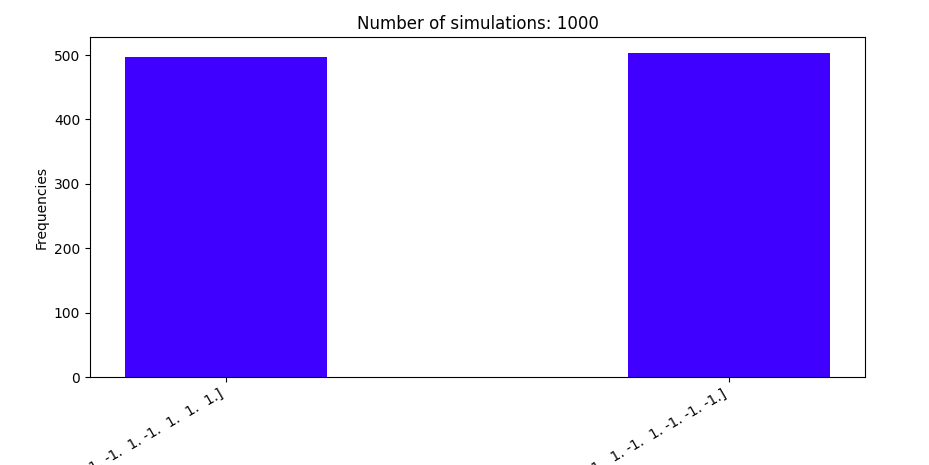
\includegraphics[scale=0.3]{img/emtracipetriple.png}
	\caption{EMT network 15 nodes}
\end{figure}
\end{frame}


\begin{frame}
\begin{figure}[H]

	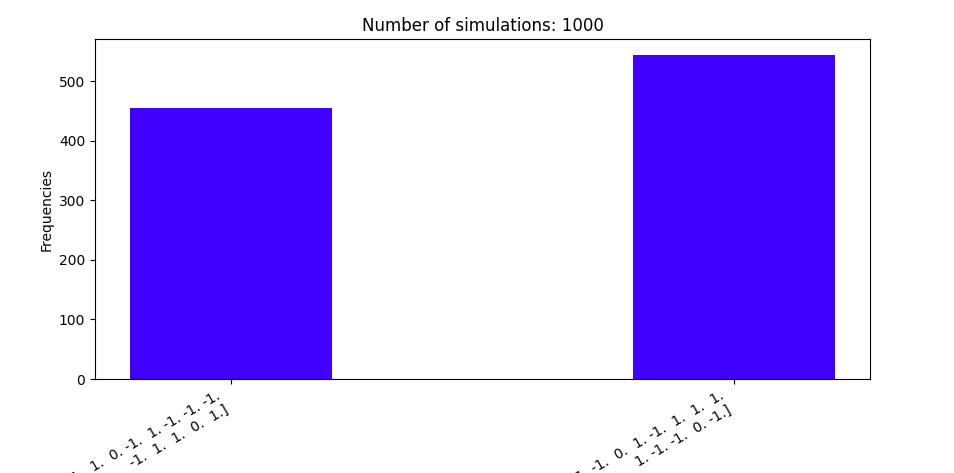
\includegraphics[scale=0.3]{img/emtracipe2terenary.png}
	\caption{EMT network 23 nodes}
\end{figure}
\end{frame}
\end{document}

